\documentclass[a4paper,11pt]{article}
\usepackage{graphicx}
\usepackage[utf8]{inputenc}
\usepackage{hyperref}

\usepackage{minted}


\hypersetup{
    colorlinks=true,
    linkcolor=blue,
    filecolor=black,      
    urlcolor=blue,
    citecolor=black,
}
\begin{document}

\title{
  \textbf{HP35 Calculator Report.}
}
\author{Adrian Jonsson Sjödin}
\date{Fall 2022}

\maketitle

\section*{Introduction}
The goal of this assignment is to evaluate how the time complexity changes when we apply different searching algorithms, as opposed to simply
searching through an array from start to end.
\section*{Task 1}

Set up a benchmark for the given method that searches through an unsorted array, and determine the relationship of how the time increases for a 
growing number of elements in the array. 

\section*{Method}

The method to benchmark was already given and required no further modification. What was left to implement for this task was solely the benchmarking 
of the given method. The implementation of this can be seen in the code bellow.

\begin{minted}[]{java}
public static double benchmarkUnsortedSearch(int maxArraySize) {
  Random rnd = new Random();
  int[] arrayToSearch = new int[maxArraySize];
  double sum = 0;
  for (int i = 0; i < 100_000; i++) {
    int key = rnd.nextInt(maxArraySize);
    long timeStart = System.nanoTime();
    searchUnsorted(arrayToSearch, key);
    sum += (double) (System.nanoTime() - timeStart) ;
  }
  return sum / 100_000;
}
\end{minted}

\section*{Result}
To benchmark the different stacks we measured the best time out of $n$ runs that it took for the calculator to
calculate an expression with 500 values followed by 499 add operations.
\begin{figure}
  \centering
  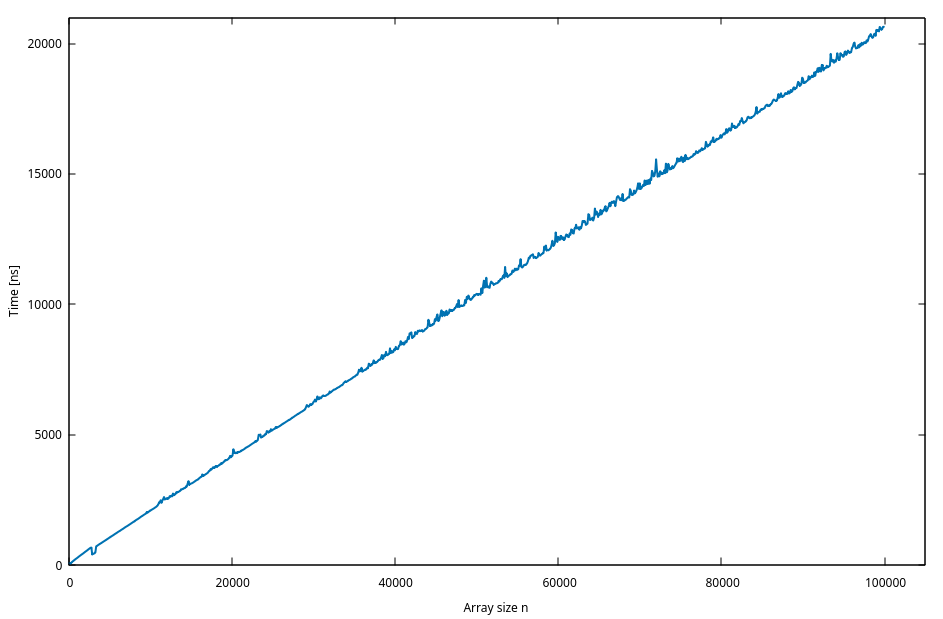
\includegraphics[width=\textwidth]{unsortedSearch.png}
  \caption{Unsorted Search}
  \label{fig:unsortedSearch}
\end{figure}


\section*{Discussion}

In plot \ref{fig:unsortedSearch} we can clearly see that the time complexity for the unsorted search was $\mathcal{O}(n)$. This was expected since
the searching algorithm will have to go through each element from element $0$ up to element $n$, which is an operation of time complexity 
$\mathcal{O}(n)$. 

The reason why I measured the average time for a search in the benchmark test is because I generated a random key to search for each time, and 
if I would have taken just the shortest amount of time it took to find said key then the result would be about the same no matter the size of the
array. This  since it is highly likely that out of the $100,000$ runs of the search algorithm for each array size, a key with a value close to, or
the same as, index $0$ would be generated. This taking the average will give a result that more accurately reflects reality.

\section*{Task 2}

Using the sorting method provided examine how long it will take to find a random key in a sorted array. Furthermore estimate how long time it would 
take to search through an array of a million entries.
\section*{Method}



\section*{Discussion}

\end{document}
